\documentclass[10pt,xcolor={dvipsnames}]{beamer}
\usetheme[progressbar=frametitle]{PaloAlto}
\usepackage{appendixnumberbeamer}
\usepackage{booktabs}
\usepackage[scale=2]{ccicons}
\usepackage{pgfplots}
\usepgfplotslibrary{dateplot}
\usepackage[utf8]{inputenc}
\usepackage{fancyvrb}
\usepackage{xspace}
\newcommand\tab[1][1cm]{\hspace*{#1}}
\usepackage{pgf-pie}
\usepackage{color}

\title{Proyecto 1}
\subtitle{Un generador de Scanners}
\date{}
\author{
    José Ceciliano Granados\newline 2016087245
    \newline \newline
    Audra Rodríguez Mora \newline 2015101893
    \newline \newline
    David Valverde Zuñiga \newline 200922986
}
\institute{Instituto Tecnológico de Costa Rica
    \newline Compiladores e Intérpretes
    \newline I Semestre 2019 }
}

\begin{document}

    \maketitle

    \begin{frame}{Tabla de contenidos}
		\setbeamertemplate{section in toc}[sections numbered]
		\tableofcontents[hideallsubsections]
	\end{frame}


    \section{Introducción}
        \begin{frame}[fragile]{Introducción}
        \begin{alertblock}{Introducción}
                Flex es una herramienta de análisis lexico desarrollada para la generación de Scanners de lenguajes. Su nombre significa "fast lexical analyzer generator". Es la alternativa gratis y open-source a la herramienta "lex".
        \end{alertblock}
        \end{frame}


    \section{Scanning}
        \begin{frame}[fragile]{Scanning}
            \begin{alertblock}{Scanning}
                El proceso de Scanning es el proceso por el cual se identifican los diferentes lexemas de un lenguaje. El proceso es tan simple como la ejecución de un Automata Deterministico Finito. Para la generación del Scanner con Flex se utilizan las expresiones regulares, conocidas como `RegEx', para indicarle a Flex que construya apartir de las expresiones regulares un DFA en C, el cual luego se usa para adquirir los diferentes lexemas del lenguaje que se planea `Scannear'.
            \end{alertblock}
        \end{frame}


    \section{Gráficos}
        \begin{frame}[fragile,allowframebreaks]{Histograma}
        \begin{alertblock}{Histograma}
            A continuación se presenta un histograma el cual indica cuantas veces cada token fue encontrado cada 50 lineas, en el \textit{axis y} se puede ver la cantidad de ocurrencias mientras en el \textit{axis x} se muestra en cual rango de lineas de codigo sucedieron.
            \end{alertblock}
        \end{frame}

    \subsection{Gráfico Barras}
        \begin{frame}[fragile]{Histograma} 
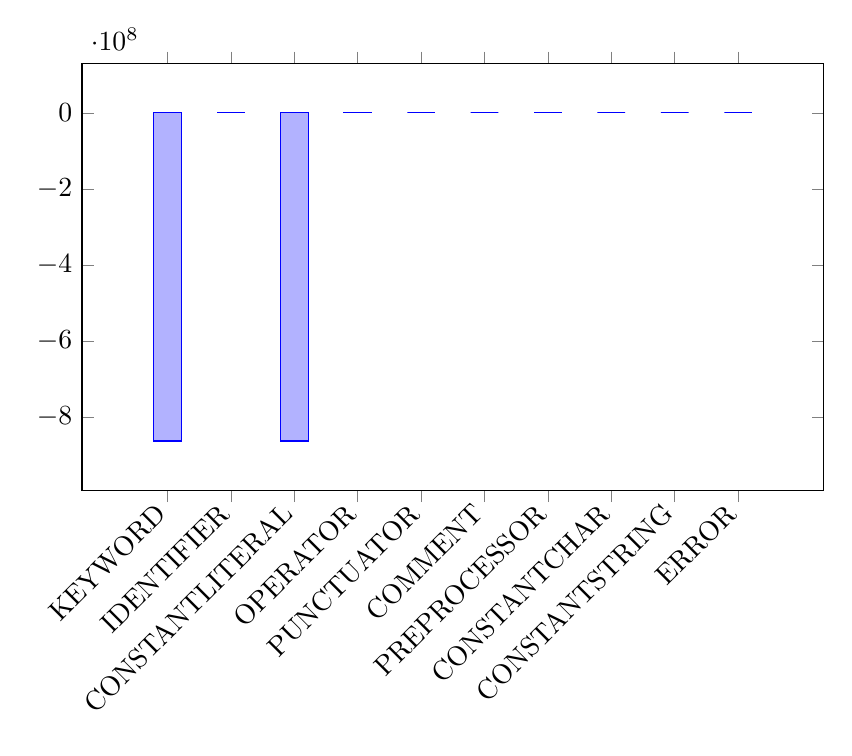
\begin{tikzpicture}     
\begin{axis}[ybar, enlargelimits=0.15, x tick label style={rotate=45, anchor=east},    symbolic x coords={KEYWORD, 
IDENTIFIER, 
CONSTANTLITERAL, 
OPERATOR, 
PUNCTUATOR, 
COMMENT, 
PREPROCESSOR, 
CONSTANTCHAR, 
CONSTANTSTRING, 
ERROR, 
},xtick=data,width=11cm,height=7cm] 
 \addplot coordinates {(KEYWORD,-863060829) 
(IDENTIFIER,32722) 
(CONSTANTLITERAL,-863060830) 
(OPERATOR,32716) 
(PUNCTUATOR,15) 
(COMMENT,0) 
(PREPROCESSOR,0) 
(CONSTANTCHAR,0) 
(CONSTANTSTRING,0) 
(ERROR,0) 
};
\end{axis}  
\end{tikzpicture} 
\end{frame}
    \subsection{Gráfico Pastel}
        \begin{frame}[fragile]{Histograma} 
\begin{tikzpicture} 
\pie[text=legend]{ 7/KEYWORD, 18/IDENTIFIER, 7/CONSTANTLITERAL, 7/OPERATOR, 47/PUNCTUATOR, 5/COMMENT, 0/PREPROCESSOR, 0/CONSTANTCHAR, 7/CONSTANTSTRING, 0/ERROR, }
\end{tikzpicture}
\end{frame}

    \section{Analisis Léxico}
        \begin{frame}[fragile,allowframebreaks]{Analisis Léxico}
        \begin{alertblock}{Codigo fuente}
            A continuación se presenta el código fuente con colores demostrando la división de Tokens.
            \end{alertblock}
        \end{frame}

        \begin{frame}[fragile,allowframebreaks]{Resaltado de sintaxis}~\newline\newline\color{Sepia}\verb$int$ \color{BlueViolet}\verb$FUNCION$\color{OliveGreen}\verb$($\color{OliveGreen}\verb$)$ \color{OliveGreen}\verb${$\newline \color{Sepia}\verb$int$ \color{BlueViolet}\verb$a$ \color{OliveGreen}\verb$=$ \color{BurntOrange}\verb$3$\color{OliveGreen}\verb$;$\newline \color{Sepia}\verb$return$ \color{BlueViolet}\verb$a$\color{OliveGreen}\verb$;$\newline\color{OliveGreen}\verb$}$\newline\newline\newline\color{Sepia}\verb$int$ \color{BlueViolet}\verb$main$\color{OliveGreen}\verb$($\color{OliveGreen}\verb$)$\color{OliveGreen}\verb${$\newline    \newline    \color{BlueViolet}\verb$FUNCION$\color{OliveGreen}\verb$($\color{OliveGreen}\verb$)$\color{OliveGreen}\verb$;$\newline    \color{Sepia}\verb$int$ \color{BlueViolet}\verb$a$ \color{OliveGreen}\verb$=$ \color{BurntOrange}\verb$9$\color{OliveGreen}\verb$;$\newline    \color{BlueViolet}\verb$a$ \color{ProcessBlue}\verb$+$\color{OliveGreen}\verb$=$ \color{BurntOrange}\verb$7$\color{OliveGreen}\verb$;$\newline\newline\newline    \color{BlueViolet}\verb$printf$\color{OliveGreen}\verb$($\color{BlueViolet}\verb$a$\color{OliveGreen}\verb$)$\color{OliveGreen}\verb$;$\newline\color{OliveGreen}\verb$}$\newline
\end{frame}



    {
        \setbeamercolor{palette primary}{fg=black, bg=yellow}
        \begin{frame}[standout]
            \begin{center}
              ¡Muchas gracias!
            \end{center}
        \end{frame}
    }

\end{document}
